%%%%%%%%%%%%%%%%%%%%%%%%%%%%%%%%%%%%%%%%%%%%%%%%%%%%%%%%%%%%%%%%%%%%%%%%%%%%
\documentclass[a4j]{jarticle}

\usepackage{jsaisig}
% \usepackage{graphicx}
\usepackage[dvipdfmx]{graphicx}

%%%%%%%%%%%%%%%%%%%%%%%%%%%%%%%%%%%%%%%%%%%%%%%%%%%%%%%%%%%%%%%%%%%%%%%%%%%

\begin{document}

% 和文タイトル
\title{Find My Matesに向けた解法の提案と実機での性能評価}

% 英文タイトル
\etitle{Solving Find My Mates and evaluation on Domestic Standard Robot}

% 著者名:
%	・各著者を\quad(全角空白)区切りで列挙
% 	・著者名の直後に\afil{所属番号}を追加→所属番号を上付で出力(\textsuperscript{所属番号}と同じ)
% 	 複数機関へ所属している場合は番号をカンマ区切りで列挙(下記著者2参照)
%  ・Corresponding Authorについては所属の後に\thanksを続け,連絡先を記入
%	・英文著者はカンマ区切りで列挙

\author{矢野 優雅\afil{1}%
	\thanks{連絡先:九州工業大学大学院生命体工学研究科人間知能システム工学専攻 \newline%
		      〒808-0135 福岡県北九州市若松区ひびきの2-4 \newline%
		      E-mail: yano.yuuga158@mail.kyutech.jp}\quad%
	福田 有輝也\afil{1}
	小野 智寛\afil{1}
	田向 権\afil{1,2}\\
	Yuga Yano\afil{1}, Yukiya Fukuda\afil{1}, Tomohiro Ono\afil{1}, and Hakaru Tamukoh\afil{1,2}}

% 所属
\affiliation{%
	\afil{1} 九州工業大学大学院生命体工学研究科\\
	\afil{1} Graduate School of Life Science and Systems Engineering, Kyushu Institute of Technology, Japan\\
	\afil{2} ニューロモルフィックAIハードウェア研究センター\\
	\afil{2} Research Center for Neuromorphic AI Hardware, Kyushu Institute of Technology, Japan}

\abstract{
Abstract (English) comes here.......................................................
}

\maketitle
\thispagestyle{empty}

%%%%%%%%%%%%%%%%%%%%%%%%%%%%%%%%%%%%%%

\section{序論}
% テストと競技表記ゆれが起きそうなので,早いうちに確定させる
\subsection{RoboCup@Home}
RoboCup@Homeは,ホームサービスロボットの技術発展を目的に開催されている競技会である.
本競技会では,人間とロボットの協調を目標の一つに掲げており,
音声認識や物体認識,ナビゲーションといった動的環境におけるテストが行われている,
そのため,より現実環境を想定した性能評価をすることができ,非常に注目を集めているリーグとなっている.
% The RoboCup@Home league aims to develop service and assistive robot technology with high relevance for future personal domestic applications. It is the largest international annual competition for autonomous service robots and is part of the RoboCup initiative. A set of benchmark tests is used to evaluate the robots’ abilities and performance in a realistic non-standardized home environment setting. Focus lies on the following domains but is not limited to: Human-Robot-Interaction and Cooperation, Navigation and Mapping in dynamic environments, Computer Vision and Object Recognition under natural light conditions, Object Manipulation, Adaptive Behaviors, Behavior Integration, Ambient Intelligence, Standardization and System Integration. It is colocated with the RoboCup symposium.
RoboCup@Homeには,Open Platform,Domestic Standard Platform(DSPL),Social Standard Platformという3つのリーグがある.
私たちの参加しているDSPLでは,トヨタ社が開発したHuman Support Robot(HSR)を標準機に採用しテストを行っている.
図\ref{overview_hsr}に,HSRの外観と搭載されているデバイスを示す.
\begin{figure}[ht]
  \centering
  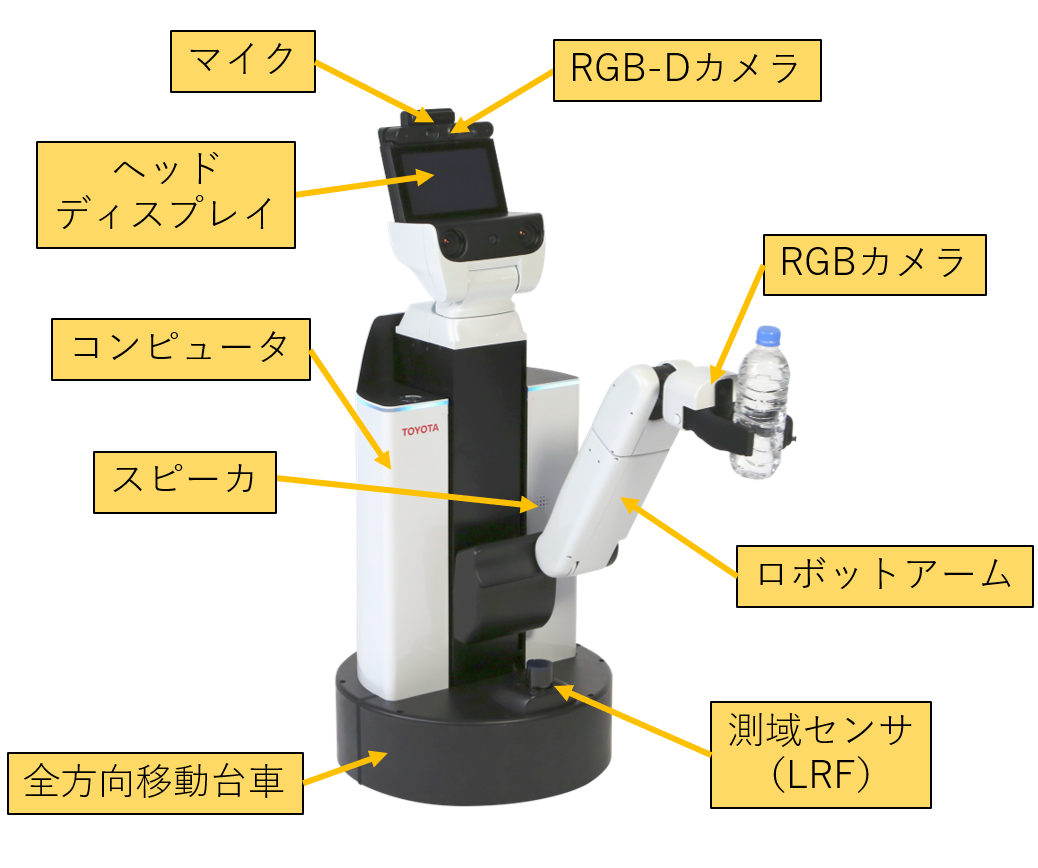
\includegraphics[width=6cm]{images/hsr/hsr_explain_ja.png}
  \caption{トヨタ社が開発したHSR}
  \label{overview_hsr}
\end{figure}
HSRは移動台車やアームに加えて,RGB-Dカメラやマイクが搭載されており,認識を通して多様なヒューマンインタラクションを行うことができる.

本研究では,ヒューマンインタラクションの性能をはかるFind My Matesというテストに向けて,その解法を提案するとともに,HSRへの実機実装を行いRoboCup@Homeでの性能評価を行う.

\subsection{Find My Mates}
本章では,RoboCup@Homeで行われるFind My Mates(FMM)というタスクについて述べる.
FMMでは,4人のゲストが1人のホストを訪れたという状況を想定している.
% しかし,ホストはゲストの名前のみを知っているがその他の情報は何も知らない.
FMMは,1人のホストの家に訪れた4人のゲストをロボットが探し,その場所,名前に加えて人物の特徴をホストに報告するというタスクである.
そのため,人物を3次元的に認識する技術と,それぞれのゲストの特徴を抽出する属性推定の技術が必要になる.
更に,ロボットは事前にゲストの名前を知らされていないため,音声認識を通してゲストの名前を知る必要がある.


\section{関連研究}


\section{提案手法}

\subsection{音声認識}
近年ではスマートフォンなどの普及により,Siriなどのクラウドを用いた音声認識の精度が非常に高くなっている.
しかし,RoboCup@Homeでは会場のネットワークが不安定である場合が想定され,安定したクラウド上での音声認識が困難である.
また,ネットワークの課題は一般の家庭環境においても想定されるものであり,オフラインでの音声認識技術を利用することは非常に有効である.
そこで本研究では,vosk\cite{vosk_hp}と呼ばれるオフラインの手法を用いて音声認識を行う.

\subsubsection{辞書設定}


\subsection{ノイズ除去}
RoboCup@Homeは実際の家庭環境を模したフィールドで行われるが,実際の家庭環境と異なる点もある.
その一つが,周囲のノイズが大きいことである.
RoboCup@Homeの他にも,サッカーリーグやレスキューリーグが同時に行われているため,実際の家庭環境では起きないような大きなノイズが発生する.
本研究では,音声認識の精度を高めるために,ノイズ除去\cite{sainburg2020finding}を音声認識の前段に組み込み,精度を高めている.


\subsection{人物認識}


\begin{table}[h]
  \centering
  \caption {表の挿入例.}
  \label{table:ex1}
  \begin{tabular}{c|cc}
    \hline
           & $a_1$ & $a_2$ \\ \hline
    $x_1$  &  0.1  &  0.1  \\
    $x_2$  &  0.2  &  0.2  \\ \hline
  \end{tabular}
\end{table}
%
□□□□□□□□□□□□□□□□□□□□
□□□□□□□□□□□□□□□□□□□□
....

図表の参照例:図\ref{fig:ex1},表\ref{fig:ex1}

参考文献の引用例:\cite{Sample1}\cite{Sample2}

%%%%%%%%%%%%%%%%%%%%%%%%%%%%%%%%%%%%%%

\section{性能評価}


\section{結論}
□□□□□□□□□□□□□□□□□□□□
□□□□□□□□□□□□□□□□□□□□
....

%%%%%%%%%%%%%%%%%%%%%%%%%%%%%%%%%%%%%%

\section*{謝辞}

□□□□□□□□□□□□□□□□□□□□
□□□□□□□□□□□□□□□□□□□□
....

%%%%%%%%%%%%%%%%%%%%%%%%%%%%%%%%%%%%%%

\begin{thebibliography}{99}
%\small

\bibitem{vosk}
Author, A., Author, B.:
JSAI SIGs Conference Paper Format Sample,
{\it International Journal of Examples}, Vol.~19, No.~4, pp.~1--2 (2007)

\bibitem{yolo}
第一著者, 第二著者:
人工知能学会研究会原稿フォーマットサンプル,
{\it International Journal of Examples}, Vol.~19, No.~4, pp.~1--2 (2007)

\bibitem{vosk_hp}
https://alphacephei.com/vosk/


\bibitem{sainburg2020finding}
Sainburg, T., Thielk, M., and Gentner, T. Q.,
% Sainburg, Tim and Thielk, Marvin and Gentner, Timothy Q
“Finding, visualizing, and quantifying latent structure across diverse animal vocal repertoires,”
{\it Public Library of Science PLoS computational biology},
Vol.16,
No.10,
pp.e1008228,
2020.

\end{thebibliography}

\end{document}
